% Very simple template for lab reports. Most common packages are already included.
\documentclass[a4paper, 11pt]{article}
\usepackage[utf8]{inputenc} % Change according your file encoding
\usepackage{graphicx}
\usepackage{indentfirst}
\usepackage{url}
\usepackage{float}
\usepackage[T1]{fontenc}

%opening
\title{%
Project Report: Key Value Web Server \\
\large Distributed Systems. Advanced Course.}
\author{Sofia Krylova <krylova@kth.se>, Iosif Koen <iosif@kth.se>}
\date{\today{}}

\begin{document}

\maketitle

\section{Introduction}
In this course, as a mandatory obligation, we were asked to implement a project from some provided projects by the course's TA. The project's main goal was to give us a better hands-on understanding of the theory components. And more specifically, the OmniPaxos algorithm and Consensus. As also, the parts like Leader election and networking include all these theoretical parts under hands-on circumstances giving us the opportunity to build our own system from scratch and letting us understand in more depth all these fascinating theoretical parts.
\section{Main problem}

In this project, we were supposed to build a web server that is made fault-tolerant using omnipaxos.
The web server should be accessed via REST or gRPC and store some data that is
accessed in a consistent manner. Furthermore, each node should maintain some statistics on
the number of requests they have handled, and we should make the node with the most requests
take over leadership when it passes a certain threshold.

\section{Solutions and Evaluation}
\subsection{Modules}
We used six classes, namely kv.rs, kv\_controler.rs, servers.rs, storage.rs, util.rs and our main.rs.
Each of these classes serves a specific utility of the web\_server.
Additionally, for these classes, we use the controller\_test.rs function under the test folder.
\subsection{util.rs}
The \verb|utils.rs| module defines several constants which are used in the project, specifically for buffering and timing.
Those constants are:
\begin{verbatim}
use std::time::Duration;

pub const BUFFER_SIZE: usize = 10000;
pub const ELECTION_TIMEOUT: Duration = Duration::from_millis(100);
pub const OUTGOING_MESSAGE_PERIOD: Duration = Duration::from_millis(100);

pub const WAIT_LEADER_TIMEOUT: Duration = Duration::from_millis(500);
pub const WAIT_DECIDED_TIMEOUT: Duration = Duration::from_millis(250);
\end{verbatim}

\begin{itemize}
    \item The \verb|BUFFER_SIZE| is a \verb|usize| constant with a value of 10,000, representing the buffer size for network communications.
    \item The \verb|ELECTION_TIMEOUT| is a Duration constant set to 100 milliseconds. This is the duration before a new election is triggered in the Paxos system if a leader is not detected.
    \item The \verb|OUTGOING_MESSAGE_PERIOD| is a Duration constant, which is set to 100 milliseconds. This duration indicates the interval at which outgoing messages are sent by the Paxos system.
    \item The \verb|WAIT_LEADER_TIMEOUT| is a Duration constant also witch set to 500 milliseconds. This duration is the time the system waits for a leader to be detected before proceeding with other tasks.
    \item Last but not least the \verb|WAIT_DECIDED_TIMEOUT| is a Duration constant set to 250 milliseconds. This duration is the time the system waits for a decision on a key-value pair before checking again.
\end{itemize}
\par
The project uses these constants to ensure consistent timing and buffering settings. They help manage the behavior of the distributed Paxos system, ensuring that elections, message sending, and decision-making are handled with appropriate timing.


\subsection{kv.rs and kv\_controler.rs}
The kv.rs module is responsible for creating a key-value store that allows for easy access and modification of data. To ensure thread safety, it uses a HashMap and a mutex. Moreover, it also incorporates a Snapshot trait that enables the creation and merging of snapshots of the key-value store.\par
We used the \verb|fn get_storage()|method that returns an \verb|Arc<Mutex<KVStore>>|

\begin{verbatim}
 pub(crate) fn get_storage() -> Arc<Mutex<KVStore>> {
        unsafe {
            match KV_STORE {
                None => {
                    let kv_store = Arc::new(Mutex::new(KVStore {
                        key_value: HashMap::new(),
                        decided_idx: 0,
                    }));
                    KV_STORE = Some(kv_store.clone());
                    kv_store
                }
                Some(ref kv_store) =>
                    kv_store.clone(),
            }
        }
    }
    
\end{verbatim}

\par
The module kv\_controller.rs is in charge of managing HTTP requests that are linked to the key-value store in a Rust-based web application that utilizes Actix Web, a well-known Rust web framework. Its primary function is to offer two API endpoints that allow for creating and retrieving key-value pairs. No crucial information is left out in this paraphrased text.

To obtain a value for a specific key from the store, we use the \verb|get(key: Path<String>)|, a GET request can be made to /key-value/{key}. The URL path should include the key parameter, and the response will provide a KeyValueResponse structure or a \verb|"404 Not Found"| status if the key is not found in the store. It is necessary to include the key parameter in the URL path to retrieve the value for that specific key.
\begin{verbatim}
    #[get("/key-value/{key}")]
pub async fn get(key: Path<String>) -> HttpResponse {
    let response = get_kv(key.into_inner()).await;

    return if response.key.is_empty() {
        HttpResponse::NotFound()
            .content_type("application/json")
            .status(StatusCode::NOT_FOUND)
            .finish()
    } else {
        HttpResponse::Ok()
            .content_type("application/json")
            .status(StatusCode::OK)
            .json(response)
    };

\end{verbatim}

\subsection{servers.rs}
The servers.rs component describes an OmniPaxos server that utilizes the Paxos distributed consensus algorithm through the OmniPaxos library. This server is responsible for managing node communication, processing incoming messages, and dispatching outgoing messages.
\par
The OmniPaxos server is executed in a continuous loop by the \verb|run()| method, which operates in an asynchronous manner. This method employs two tokio intervals - \verb|election_interval| for managing election timeouts and \verb|outgoing_interval| for transmitting outgoing messages. Additionally, it monitors the incoming Receiver channel for any new messages and handles them by utilizing the \verb|handle_incoming()| function of the \verb|omni_paxos| instance.
\begin{verbatim}
pub(crate) async fn run(&mut self) {
    let mut outgoing_interval = time::interval(OUTGOING_MESSAGE_PERIOD);
    let mut election_interval = time::interval(ELECTION_TIMEOUT);
    loop {
        tokio::select! {
            biased;
            _ = election_interval.tick() => { self.omni_paxos.lock()
            .unwrap()
            .election_timeout(); },
            _ = outgoing_interval.tick() => { self.send_outgoing_msgs().await; },
            Some(in_msg) = self.incoming.recv() => { self.omni_paxos.lock()
            .unwrap()
            .handle_incoming(in_msg); },
            else => { }
        }
    }
}
\end{verbatim}
\par
The function \verb|configure_persistent_storage()| requires a String type path as input and produces a \verb|PersistentStorageConfig| object as output. It operates by generating a \verb|LogOptions| object and a \verb|sled::Config| object using the path provided, which it then utilizes to create a default \verb|PersistentStorageConfig|.
\begin{verbatim}
      pub(crate) fn configure_persistent_storage(path: String) -> 
      PersistentStorageConfig {
        let log_opts = LogOptions::new(path.clone());
        let mut sled_opts = Config::new();
        sled_opts = Config::path(sled_opts, path.clone());

        // generate default configuration and set user-defined options
        let persist_config = PersistentStorageConfig::with(
            path.to_string(), log_opts, sled_opts);

        persist_config
    }
}
\end{verbatim}
\par
The servers.rs module provides the necessary structure and methods to run an OmniPaxos server, manage communication between nodes in the network, and handle timeouts and message processing.
\subsection{storage.rs}

The management of \verb|key-value storage|, including the creation and retrieval of key-value pairs, as well as synchronization between local storage and the distributed Paxos system, is handled by the \verb|storage.rs| module.
\par
The \verb|sync_decided_kv()| method is responsible for synchronizing the local key-value storage with the distributed Paxos system. This function locks the \verb|KVStore| and selects a server from \verb|OP_SERVER_HANDLERS| randomly. Afterward, it retrieves the decided entries from the server and updates the local \verb|key-value storage|. This method ensures that both snapshotted entries and decided entries are appropriately handled.
\begin{verbatim}
async fn sync_decided_kv() {
    let kv_store = KVStore::get_storage();
    let mut storage = kv_store.lock().unwrap();

    let handler = OP_SERVER_HANDLERS.lock().unwrap();
    let server_id = rand::thread_rng().gen_range(1..PEERS);
    // println!("Chosen server {}", server_id);
    let (server, _, _) = handler.get(&server_id).unwrap();

    let last_idx = server
        .lock()
        .unwrap()
        .get_decided_idx();
    println!("Last index {}", last_idx);
    println!("Local index {}", storage.decided_idx);

    let mut overlap = false;
    if storage.decided_idx == 0 { overlap = true; }
    if last_idx > storage.decided_idx {
        let committed_ents = server
            .lock()
            .unwrap()
            .read_decided_suffix(storage.decided_idx as u64)
            .expect("Failed to read expected entries");

        for (_, ent) in committed_ents.iter().enumerate() {
            match ent {
                LogEntry::Decided(kv_decided) => {
                    storage.decided_idx += 1;
                    storage.key_value.insert(kv_decided.key
                    .clone(), kv_decided.value);
                    println!("Adding value: {:?}, decided idx {} via server {}",
                             kv_decided.value, storage.decided_idx, server_id);
                }
                LogEntry::Snapshotted(kv_snapshotted) => {
                    for (k, v) in &kv_snapshotted.snapshot.snapshotted {
                        storage.decided_idx += 1;
                        storage.key_value.insert(k.clone(), *v);
                        println!("Adding value: {:?}, decided inx {} via server {}",
                                 v, storage.decided_idx, server_id);
                    }
                }
                _ => {} // ignore not committed entries
            }
        }
    }
\end{verbatim}
\par
Overall the storage.rs module provides the functions to create and retrieve key-value pairs while ensuring that the local key-value storage is synchronized with the distributed Paxos system. This allows for consistent and \verb|fault-tolerant key-value| storage across a distributed network.

\subsection{main.rs}
The \verb|main.rs| module is as its name says our main program and serves as the entry point for the application of \verb|server|. It sets up the OmniPaxos \verb|key-value| store, initializes the servers, and starts the HTTP server. The HTTP server exposes two routes for creating and getting \verb|key-value| pairs.\par
Firstly let's see the \verb|main()| function witch sets up the environment and starts the HTTP server. It first calls the \verb|cleanup()| function to remove any previous storage directories. Next, it initializes the OmniPaxos servers and handlers by calling \verb|initialise_handlers()|. Finally, it starts the Actix HTTP server with two routes for creating and getting key-value pairs.
\begin{verbatim}
async fn main() -> std::io::Result<()> {
    // Clean-up storage
    cleanup();

    OP_SERVER_HANDLERS
        .lock()
        .unwrap()
        .extend(initialise_handlers());

    HttpServer::new(move || App::new().service(create).service(get))
        .bind(("127.0.0.1", 8080))?
        .run()
        .await
}
\end{verbatim}
We can see the methods/functions in our \verb|main| module.
\begin{itemize}
    \item The \verb|cleanup()| function removes any previous storage directories.
    \item The \verb|initialise_channels()| creates sender and receiver channels for the OmniPaxos system.
    \item The \verb|initialise_handlers()| initialize the OmniPaxos servers, handlers, and configurations.
    \item Finally the \verb|recovery()| is use to recover a failed node by recreating its storage and rejoining the network.
\end{itemize}

\subsection{test.rs}
Finally, in the \verb|test.rs| module containing tests for the OmniPaxos key-value store implemented in the main application. It uses the \verb|restest| library to test the HTTP endpoints and \verb|tokio| for asynchronous execution. The tests include creating and getting key-value pairs, both individually and concurrently.
Namely, the test functions are:
\begin{itemize}
    \item \verb|test_create()|
    \item \verb|test_multiple_create()|
    \item \verb|test_get()|
\end{itemize}

\section{Run}
\par
In this section, we will explain how to run the server via your command line. First, you need to make a configuration on our \verb|main| module at the \verb|main()| function, you should check the \verb|.bind(("127.0.0.1", 8080))?| and see if the Ip and the port number are working for your machine.
\par
Then you should go to your terminal and run the \verb|cargo run| command or inside from your editor can click the button run on the \verb|main()| function. If you take a message like:\par
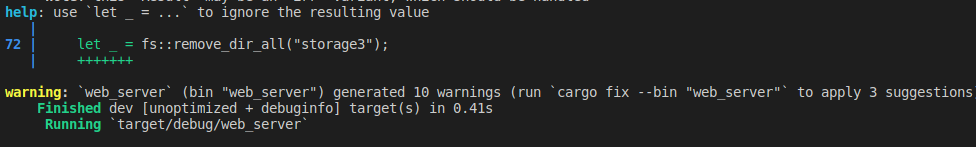
\includegraphics[width=\textwidth,keepaspectratio]{Run.png}
Then you are safe to continue and your server is up and running.
\par
Now you need to go to the \verb|tests/controler_test.rs| where you can find the test for the server and you can run the simple by clicking the run button on each of them. The preferable output is:\par
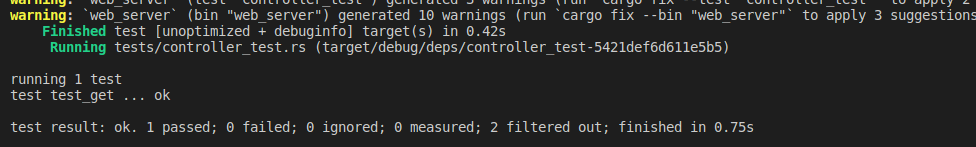
\includegraphics[width=\textwidth,keepaspectratio]{Test1.png}


\section{Conclusions}
In this last project of the course, we asked to create our own stable server. The process was exciting. We obtained new knowledge, and more importantly, we understood and saw a lot of the theory in action and the hands-on work; this gave us an excellent grasp of the course outcome knowledge.
\end{document}
